%iffalse
\let\negmedspace\undefined
\let\negthickspace\undefined
\documentclass[journal,12pt,onecolumn]{IEEEtran}
\usepackage{cite}
\usepackage{amsmath,amssymb,amsfonts,amsthm}
\usepackage{algorithmic}
\usepackage{graphicx}
\usepackage{textcomp}
\usepackage{xcolor}
\usepackage{txfonts}
\usepackage{listings}
\usepackage{enumitem}
\usepackage{mathtools}
\usepackage{gensymb}
\usepackage{comment}
\usepackage[breaklinks=true]{hyperref}
\usepackage{tkz-euclide} 
\usepackage{listings}
\usepackage{gvv}                                        
%\def\inputGnumericTable{}                                 
\usepackage[latin1]{inputenc}     
\usepackage{xparse}
\usepackage{color}                                            
\usepackage{array}                                            
\usepackage{longtable}                                       
\usepackage{calc}                                             
\usepackage{multirow}
\usepackage{multicol}
\usepackage{hhline}                                           
\usepackage{ifthen}                                           
\usepackage{lscape}
\usepackage{tabularx}
\usepackage{array}
\usepackage{float}
\newtheorem{theorem}{Theorem}[section]
\newtheorem{problem}{Problem}
\newtheorem{proposition}{Proposition}[section]
\newtheorem{lemma}{Lemma}[section]
\newtheorem{corollary}[theorem]{Corollary}
\newtheorem{example}{Example}[section]
\newtheorem{definition}[problem]{Definition}
\newcommand{\BEQA}{\begin{eqnarray}}
\newcommand{\EEQA}{\end{eqnarray}}
\usepackage{float}
\usepackage{listings}
\usepackage{xcolor}
%\newcommand{\define}{\stackrel{\triangle}{=}}
\theoremstyle{remark}
\usepackage{ circuitikz }
%\newtheorem{rem}{Remark}
% Marks the beginning of the document
\begin{document}
\title{10.4.1.2.3}
\author{EE24BTECH11007 - Arnav Makarand Yadnopavit}
\maketitle
\renewcommand{\thefigure}{\theenumi}
\renewcommand{\thetable}{\theenumi}
\parindent 0px Question: Rohan's mother is 26 years older than him. The product of their ages (in years)
3 years from now will be 360. We would like to find Rohan's present age.\\
\solution\\
\textbf{Theoretical Solution:}\\
Let Rohan's age, R=$x$.\\
Then Mother's age, M=$x+26$
Then after 3 years we get
\begin{align}
    \brak{M+3}\brak{R+3}&=360 \label{eq:f}\\
    \brak{x+29}\brak{x+3}&=360\\
    x^2+32x-273&=0\\
\end{align}
Solving the equation we get, $x=7$ or $x=-39$. Eliminating $x=-39$ (Age considered to be a non-negative value)\\
Rohan's present age is 7.\\ 
\textbf{Computational Solution:}\\
Two methods for finding the solution of a quadratic equation are:\\
Matrix-Based Method:\\
For a polynomial equation of form $x^n+b_{n-1}x^{n-1}+\dots+b_2x^2+b_1x+b_0 = 0$ we construct a matrix called companion matrix of form
\begin{align}
	\Lambda = \myvec{0&1&0&\dots&0\\ 0&0&1&\dots&0\\ \vdots &\vdots &\vdots &\ddots&\vdots\\0&0&0&\vdots&1\\-b_0&-b_1&-b_2&\dots&-b_{n-1}}
\end{align}
The eigenvalues of this matrix are the roots of the given polynomial equation.\\
\textbf{Finding eigenvalues}
\section{QR Algorithm with Householder technique and Wilkinson Shift}
\subsection{QR Decomposition}
QR decomposition factors a given matrix $A$ into:
$$A = QR,$$
where $Q$ is an orthogonal matrix $\brak{Q^\top Q = I}$, and $R$ is an upper triangular matrix.

\subsection{Householder Transformations}
Householder transformations are used to zero out elements below the diagonal of a matrix column. Given a vector $v$, the Householder matrix is:
\begin{align}
    H = I - 2\frac{vv^\top}{v^\top v}
\end{align}
The way it works is:\\
Initialize Q as Identity matrix. Let $\vec{x}$ be the the first column of $A$, and $\alpha=\norm{\vec{x}}$.\\
\begin{align}
    \vec{u}&=\vec{x}-\alpha\vec{e_1}\\
    \vec{v}&=\frac{\vec{u}}{\norm{\vec{u}}}\\
    Q&=I-2vv^H
\end{align}
By this we obtain $Q_1$ such that:\\
$$Q_1A=\myvec{\alpha_1 & * & \dots & *\\ 0 & & &\\\vdots & & A^\prime &\\0 & & &}$$
This can be repeated for $A^\prime$ (obtained from $Q_1A$ by deleting the first row and first column), resulting in a Householder matrix $Q^\prime_2$. Note that $Q\prime_2$ is smaller than $Q_1$. Since we want it really to operate on $Q_1A$ instead of $A^\prime$ we need to expand it to the upper left, filling in a 1, or in general:
$$Q_k=\myvec{I_{k-1} & 0 \\ 0 & Q^\prime_k}$$\\
After $n-1$ iterations of this process.\\
\begin{align}
R=Q_{n-1}\dots Q_2Q_1A\\
Q^\top=Q_{n-1}\dots Q_2Q_1\\
Q=Q_1Q_2\dots Q_{n-1}
\end{align}
\subsection{QR Algorithm for Eigenvalues}
The QR algorithm iteratively applies QR decomposition to a shifted matrix \( A - \mu I \) and reconstructs it as:
$$A = RQ + \mu I$$
converging to an upper triangular form with eigenvalues on the diagonal.\\
where $\mu$ can be calculated by:\\
$$\mu=a_m-\frac{\delta}{\abs{\delta}}\frac{b^2_{m-1}}{\abs{\delta}+\sqrt{\delta^2+b^2_{m-1}}}$$
where B is the lower rightmost $2\times 2$ matrix of $A$, B= \myvec{a_{m-1}&b^\prime_{m-1}\\b^\prime_{m-1}&a_m}\\
$\delta=\frac{a_{m-1}-a_m}{2}$\\
If $\delta=0$, then $\mu=a_m-b_{m-1}$
\subsection{Complex Eigenvalues}
In case a matrix has complex eigenvalues a hessenberg matrix $\brak{2\times2}$ will be formed along the diagonal of the triangularised matrix A such that:
$$A=\myvec{\lambda_1 & \dots & \dots & \dots \\ 0 & a & b & \dots\\ \vdots & c & d & \dots\\ 0 & \dots & \dots & \lambda_n}$$
then:
\begin{align*}
    \lambda_2=\frac{a+d+\sqrt{\brak{a+d}^2-4\brak{ad-bc}}}{2}\\
    \lambda_3=\frac{a+d-\sqrt{\brak{a+d}^2-4\brak{ad-bc}}}{2}\\
\end{align*}
The solution given by the code is
\begin{align}
	x_1=7.000000 + 0.000000i\\
    x_2=-39.000000 + 0.000000i
\end{align}
\textbf{Newton-Raphson Method:}\\
Start with an initial guess $x_0$, and then run the following logical loop,
\begin{align}
    x_{n+1} = x_n - \frac{f\brak{x_n}}{f^{\prime}\brak{x_n}} 
\end{align}
where,
\begin{align}
    f\brak{x} = x^2 + 32x - 273\\
    f^{\prime}\brak{x} = 2x-32
\end{align}
The update equation will be
\begin{align}
	x_{n+1} = x_n - \frac{2{x_n}^2 - 13x_n + 9}{4x_n-13}\\
\end{align}
The problem with this method is if the roots are complex but the coefficients are real, $x_n$ either converges to an extrema or grows continuously without any bound.
However, to obtain complex solutions, we can just take the initial guess point to be a
random complex number.\\
The output of a program written to find roots is shown below:
\begin{align}
	r_1 = 0.7878\\
	r_2 = 5.7122
\end{align}
\begin{figure}[h]
    \centering
    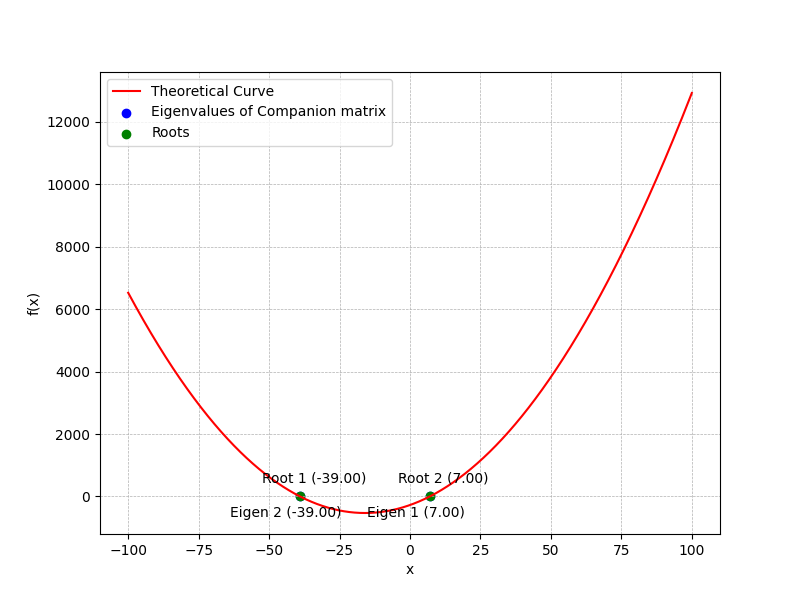
\includegraphics[width=\columnwidth]{figs/fig.png}
 \end{figure}
\end{document}

